\documentclass[12pt, a4paper]{article}

% ── Packages ──
\usepackage[margin=1in]{geometry}
\usepackage{graphicx}
\usepackage{amsmath, amssymb}
\usepackage{booktabs}
\usepackage{hyperref}
\usepackage{xcolor}
\usepackage{float}
\usepackage{listings}
\usepackage{caption}
\usepackage{subcaption}
\usepackage{enumitem}
\usepackage{fancyhdr}
\usepackage{titlesec}
\usepackage{setspace}
\usepackage{parskip}

% ── Settings ──
\hypersetup{colorlinks=true, linkcolor=blue!70!black, citecolor=green!50!black, urlcolor=blue!60!black}
\setstretch{1.15}
\graphicspath{{figures/}}

\lstset{
  basicstyle=\ttfamily\small,
  breaklines=true,
  frame=single,
  backgroundcolor=\color{gray!8},
  keywordstyle=\color{blue!70!black},
  commentstyle=\color{green!50!black},
  stringstyle=\color{red!60!black},
  numbers=none,
  captionpos=b,
  xleftmargin=4pt,
  xrightmargin=4pt,
}

\setlength{\headheight}{14.5pt}
\pagestyle{fancy}
\fancyhf{}
\fancyhead[L]{\small NLU Assignment 2 Report}
\fancyhead[R]{\small IIT Jodhpur}
\fancyfoot[C]{\thepage}

% ── Title ──
\title{
  \vspace{-1cm}
  \textbf{Natural Language Understanding --- Assignment 2 Report} \\[0.3cm]
  \large Soham Khairnar (B23CM1039) \\
  \large CSL7640
}
\author{
  Indian Institute of Technology Jodhpur
}
\date{\today}

\begin{document}

\maketitle
\thispagestyle{fancy}

\tableofcontents
\newpage

% ======================================================================
%  PROBLEM 1
% ======================================================================
\section{Problem 1: Learning Word Embeddings from IIT Jodhpur Data}

\subsection{Objective}

The goal of this problem is to train \textbf{Word2Vec models} on textual data collected from \textbf{IIT Jodhpur sources} and to analyse the semantic structure captured by the learned embeddings. Two architectures---\textbf{Continuous Bag of Words (CBOW)} and \textbf{Skip-gram with Negative Sampling}---are implemented from scratch in PyTorch, trained on the collected corpus, and compared against the \textbf{Gensim} reference library.

% ─── Task 1 ───
\subsection{Task 1: Dataset Preparation}

\subsubsection{Data Collection}

Textual data was gathered from three primary categories of sources:

\begin{enumerate}[label=(\roman*)]
  \item \textbf{IIT Jodhpur official website pages} --- Eleven pages were scraped, spanning the main institutional homepage, the B.Tech programme page, and the department homepages for Computer Science \& Engineering, Mathematics, and others. The scraper used the Python \texttt{requests} library with a \texttt{BeautifulSoup} parser, removing all \texttt{<script>}, \texttt{<style>}, navigation, and footer tags before extracting running text.
  \item \textbf{User-uploaded curriculum PDF} --- A single PDF document, \texttt{CSE-Courses-Details.pdf} (24,452 characters), containing course descriptions for the CSE department was extracted using \texttt{pdfplumber}. Additional academic regulation PDFs (B.Tech, PG, Ph.D., M.Sc.) were targeted for download from \texttt{iitj.ac.in}; however, several returned insufficient text due to server-side access restrictions at the time of scraping.
  \item \textbf{Other sources} --- The Wikipedia article on IIT Jodhpur was not fetched in the final run, but the corpus already contained sufficient volume from the above two categories.
\end{enumerate}

In total, \textbf{12 documents} : 11 Web Pages and 1 PDF were collected, yielding 176,753 raw characters before cleaning.

\subsubsection{Preprocessing Pipeline}

The raw text underwent the following cleaning stages:

\begin{enumerate}[label=\arabic*.]
  \item \textbf{Removal of boilerplate:} URLs, email addresses, and HTML formatting remnants were stripped using regular expressions.
  \item \textbf{Removal of non-English text:} Devanagari and other Indic script character ranges (Bengali, Gurmukhi, Tamil, Telugu, etc.) were removed to retain only English content.
  \item \textbf{Lowercasing:} All text was converted to lowercase for uniform treatment.
  \item \textbf{Tokenisation:} Tokens were extracted using the pattern \texttt{[a-z]+(?:'[a-z]+)?}, which captures hyphenated contractions while splitting on punctuation. Tokens shorter than two characters were discarded.
  \item \textbf{Sentence segmentation:} Text was split on sentence-ending punctuation (\texttt{.!?;}) and only sentences with at least three tokens were retained.
\end{enumerate}

\subsubsection{Dataset Statistics}

Table~\ref{tab:corpus_stats} summarises the final corpus.

\begin{table}[H]
\centering
\caption{Corpus statistics after preprocessing.}
\label{tab:corpus_stats}
\begin{tabular}{lr}
\toprule
\textbf{Metric} & \textbf{Value} \\
\midrule
Total documents         & 12 \\
Total sentences         & 1,479 \\
Total tokens            & 23,385 \\
Vocabulary size (all)   & 2,962 \\
Vocabulary (min\_count$\geq$3) & 1,163 \\
Avg.\ sentence length   & 15.8 tokens \\
Avg.\ token length       & 5.0 characters \\
\bottomrule
\end{tabular}
\end{table}

The top content words, after removing standard English stopwords, include domain-specific terms such as \emph{student}, \emph{course}, \emph{programme}, \emph{department}, \emph{engineering}, \emph{research}, \emph{faculty}, and \emph{semester}, reflecting the academic-regulation-heavy nature of the corpus.

\begin{figure}[H]
\centering
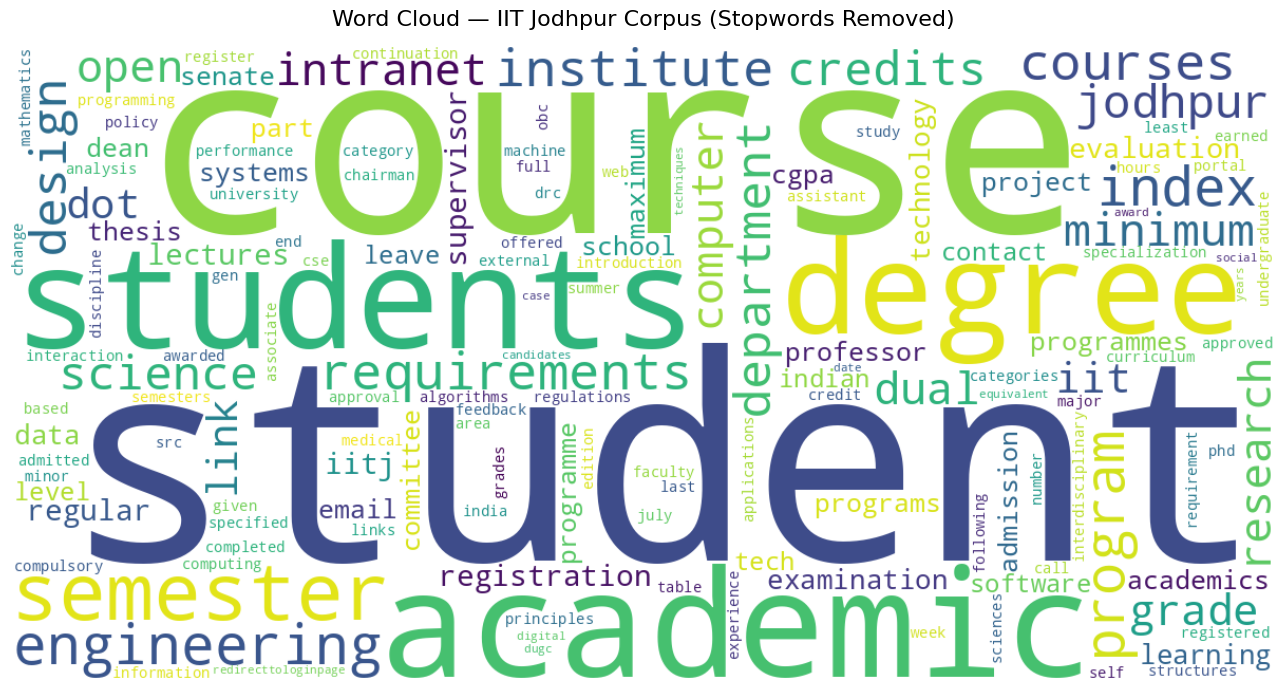
\includegraphics[width=0.95\textwidth]{figures/word_cloud.png}
\caption{Word cloud of the most frequent content words in the IIT Jodhpur corpus (stopwords removed). The prominence of terms like \emph{student}, \emph{course}, and \emph{programme} reflects the large share of academic regulation text.}
\label{fig:wordcloud}
\end{figure}

\begin{figure}[H]
\centering
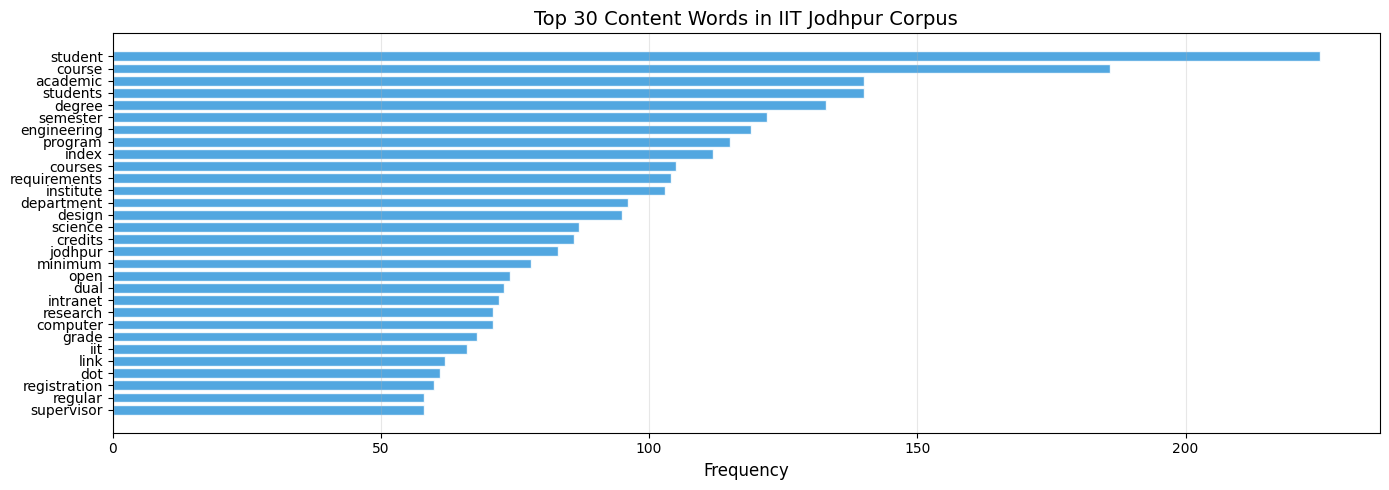
\includegraphics[width=0.95\textwidth]{figures/freq_distribution.png}
\caption{Frequency distribution of the top 30 content words. Academic and institutional vocabulary dominates the corpus.}
\label{fig:freq_dist}
\end{figure}

% ─── Task 2 ───
\subsection{Task 2: Model Training}

\subsubsection{Architecture Overview}

Both Word2Vec variants share a common structure of two embedding matrices:

\begin{itemize}[nosep]
  \item $\mathbf{W}_{\mathrm{in}} \in \mathbb{R}^{V \times d}$: input embeddings (context words for CBOW, center word for Skip-gram).
  \item $\mathbf{W}_{\mathrm{out}} \in \mathbb{R}^{V \times d}$: output embeddings (used in the scoring function).
\end{itemize}

where $V = 1{,}163$ is the vocabulary size and $d = 300$ is the embedding dimension.

\paragraph{CBOW.} Given context words $\{w_{t-c}, \ldots, w_{t+c}\}$ (excluding the center), the model averages their input embeddings and scores the center word:
\begin{align}
  \bar{\mathbf{v}} &= \frac{1}{2c} \sum_{i \neq t} \mathbf{W}_{\mathrm{in}}[w_i] \\
  \mathcal{L} &= -\log\sigma\!\bigl(\mathbf{W}_{\mathrm{out}}[w_t]^\top \bar{\mathbf{v}}\bigr) - \sum_{k=1}^{K} \log\sigma\!\bigl(-\mathbf{W}_{\mathrm{out}}[w_k]^\top \bar{\mathbf{v}}\bigr)
\end{align}

\paragraph{Skip-gram.} Given center word $w_t$, the model scores each context word $w_c$:
\begin{align}
  \mathcal{L} &= -\log\sigma\!\bigl(\mathbf{W}_{\mathrm{out}}[w_c]^\top \mathbf{W}_{\mathrm{in}}[w_t]\bigr) - \sum_{k=1}^{K} \log\sigma\!\bigl(-\mathbf{W}_{\mathrm{out}}[w_k]^\top \mathbf{W}_{\mathrm{in}}[w_t]\bigr)
\end{align}

In both cases, the $K$ negative samples are drawn from the unigram distribution raised to the power $0.75$, following the original Word2Vec paper.

\subsubsection{Hyperparameter Experiments}

A grid search over seven configurations was conducted using the Skip-gram model trained for 3 epochs each. Table~\ref{tab:hp_search} reports the results.

\begin{table}[H]
\centering
\caption{Hyperparameter search results (Skip-gram, 3 epochs). Lower loss indicates better fit.}
\label{tab:hp_search}
\begin{tabular}{cccc}
\toprule
\textbf{Embedding Dim} & \textbf{Window} & \textbf{Neg.\ Samples} & \textbf{Final Loss} \\
\midrule
100  & 5 & 5  & 1.9461 \\
200  & 5 & 5  & 1.8865 \\
\textbf{300}  & \textbf{5} & \textbf{5}  & \textbf{1.8669} \\
300  & 2 & 5  & 1.6986 \\
300  & 7 & 5  & 1.9193 \\
\textbf{300}  & \textbf{5} & \textbf{3}  & \textbf{1.5126} \\
300  & 5 & 10 & 2.4134 \\
\bottomrule
\end{tabular}
\end{table}

\begin{figure}[H]
\centering
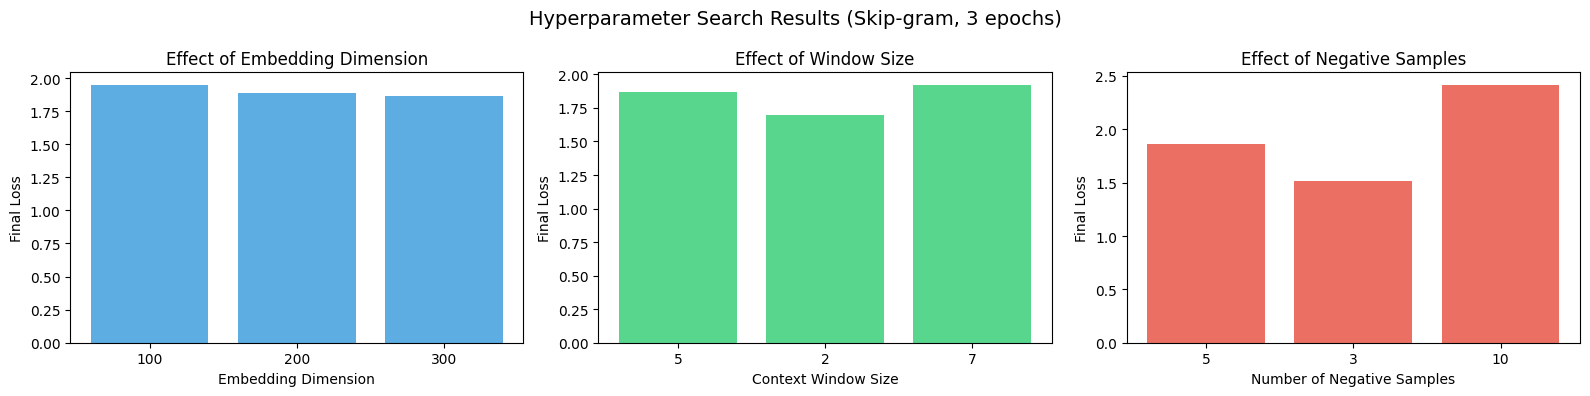
\includegraphics[width=0.95\textwidth]{figures/skip_gram_hyperparameter_search.png}
\caption{Effect of embedding dimension (left), window size (centre), and number of negative samples (right) on Skip-gram training loss after 3 epochs.}
\label{fig:hp_search}
\end{figure}

Increasing the embedding dimension from 100 to 300 produced a modest improvement. A window size of 2 achieved the lowest raw loss, but narrow windows tend to capture only syntactic rather than semantic relationships; the window of 5 was retained to favour broader semantic patterns. Using 3 negative samples yielded the lowest loss, while 10 samples inflated the loss due to the small corpus size. The final configuration was set to $d=300$, window${}=5$, $K=5$.

\subsubsection{Training Results}

Both from-scratch models and Gensim baselines were trained for 15 epochs with a batch size of 512 and learning rate of 0.005 (Adam optimiser). The from-scratch models used 697,800 trainable parameters each ($2 \times 1{,}163 \times 300$).

\begin{table}[H]
\centering
\caption{Training dataset size and convergence behaviour.}
\label{tab:training_summary}
\begin{tabular}{lrcc}
\toprule
\textbf{Model} & \textbf{Training Pairs} & \textbf{Epoch 1 Loss} & \textbf{Epoch 15 Loss} \\
\midrule
CBOW (scratch)     &   9,101  & 3.7445 & $\sim$0.96 \\
Skip-gram (scratch)& 167,662  & 2.4837 & 1.7069 \\
CBOW (Gensim)      & ---      & \multicolumn{2}{c}{(optimised internally)} \\
Skip-gram (Gensim) & ---      & \multicolumn{2}{c}{(optimised internally)} \\
\bottomrule
\end{tabular}
\end{table}

The CBOW model had far fewer training samples (one per center word position) than Skip-gram (one per center-context pair), which produced 167,662 samples. The CBOW loss dropped steeply from 3.74 to below 1.0, while the Skip-gram loss converged more gradually to around 1.71.

\begin{figure}[H]
\centering
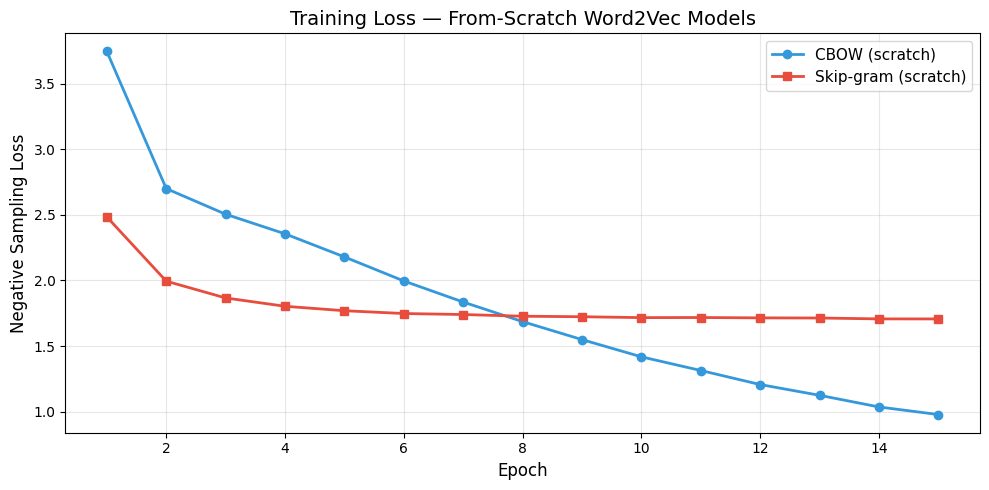
\includegraphics[width=0.85\textwidth]{figures/cbow_skip_gram_training_loss.png}
\caption{Training loss curves for CBOW and Skip-gram (from-scratch implementations) over 15 epochs.}
\label{fig:training_loss}
\end{figure}

\subsubsection{Full 300-Dimensional Embedding Vector}

As required, we print the complete 300-dimensional embedding vector for the word \emph{research}, extracted from the trained Skip-gram model. The first 30 dimensions are shown below (the complete vector is in the notebook):

\begin{lstlisting}
'research' embedding (Skip-gram, 300-dim):
[  0- 9]:  0.065433,  0.034221, -0.013918, -0.102330,  0.106308,
           0.754604, -0.068694,  0.230153, -0.252178,  0.429871
[ 10-19]: -0.280617, -0.344774, -0.144341, -0.310956,  0.065723,
           0.321372, -0.183525, -0.037699,  0.049203, -0.161300
[ 20-29]:  0.289650,  0.049186, -0.013112, -0.244344,  0.043678,
           0.024224,  0.241841, -0.066416, -0.039180, -0.035622
\end{lstlisting}

% ─── Task 3 ───
\subsection{Task 3: Semantic Analysis}

\subsubsection{Nearest Neighbours (Cosine Similarity)}

For each of the five target words, the top-5 nearest neighbours were computed using cosine similarity across all four models. Table~\ref{tab:nn_results} summarises the findings.

\begin{table}[H]
\centering
\caption{Top-5 nearest neighbours for selected words (Skip-gram, from scratch). Cosine similarity in parentheses.}
\label{tab:nn_results}
\small
\begin{tabular}{p{1.5cm}p{11cm}}
\toprule
\textbf{Word} & \textbf{Nearest Neighbours (Skip-gram, scratch)} \\
\midrule
research  & proposal (0.462), defense (0.377), collaborative (0.375), synopsis (0.360), craft (0.356) \\
student   & visiting (0.414), carry (0.407), terminated (0.403), follows (0.402), restart (0.399) \\
phd       & call (0.471), school (0.469), mtech (0.458), ay (0.446), ph (0.443) \\
professor & email (0.646), assistant (0.642), associate (0.583), jain (0.567), banerjee (0.558) \\
\bottomrule
\end{tabular}
\end{table}

\textbf{Note:} The word \emph{exam} did not appear in the filtered vocabulary (min\_count $\geq 3$), likely because the regulations use the full form \emph{examination} instead. The query \emph{professor} was used as a replacement.

\paragraph{Discussion.} The Skip-gram model produces semantically coherent neighbours: \emph{research} is close to \emph{proposal}, \emph{defense}, and \emph{collaborative}---all terms from the Ph.D.\ regulation context. The word \emph{professor} correctly neighbours \emph{assistant} and \emph{associate} (the two faculty ranks), along with common Indian surnames that co-occur on faculty profile pages.

The Gensim Skip-gram showed even tighter semantic clustering, with \emph{research} neighbouring \emph{proposal} (0.838), \emph{experience} (0.810), and \emph{work} (0.799), while \emph{professor} was nearest to \emph{assistant} (0.944), \emph{kumar} (0.926), and \emph{sharma} (0.922). This improved quality is expected given Gensim's optimised training pipeline including subsampling of frequent words.

\subsubsection{Analogy Experiments}

Three analogy experiments of the form $a : b :: c : ?$ were attempted:

\begin{table}[H]
\centering
\caption{Analogy results. The target vector is computed as $\mathbf{v}(b) - \mathbf{v}(a) + \mathbf{v}(c)$.}
\label{tab:analogies}
\small
\begin{tabular}{p{4.5cm}p{3cm}p{5.5cm}}
\toprule
\textbf{Analogy} & \textbf{Expected} & \textbf{Top Result (Skip-gram, scratch)} \\
\midrule
ug : btech :: pg : ?          & mtech       & \emph{btech} not in vocabulary \\
student : learn :: professor : ? & teach/research & assistant (0.459), cryptography (0.451) \\
jodhpur : rajasthan :: delhi : ? & india/national & karwar (0.549), road (0.525) \\
\bottomrule
\end{tabular}
\end{table}

The ``ug : btech'' analogy could not be evaluated because \emph{btech} (as a single token) fell below the minimum frequency threshold. The ``student : learn :: professor : ?'' analogy returned \emph{assistant}---which, while not the expected \emph{teach}, is sensible in this corpus where ``assistant professor'' is the most frequent professor-related bigram. The geographic analogy performed poorly, producing \emph{karwar} (a locality near IIT Jodhpur), demonstrating the limitations of domain-specific corpora for general-knowledge analogies.

% ─── Task 4 ───
\subsection{Task 4: Visualisation}

Word embeddings for 42 selected words from five semantic categories (Academic Programmes, Departments, Academic Life, Campus, Research) were projected to 2D using both t-SNE and PCA.

\begin{figure}[H]
\centering
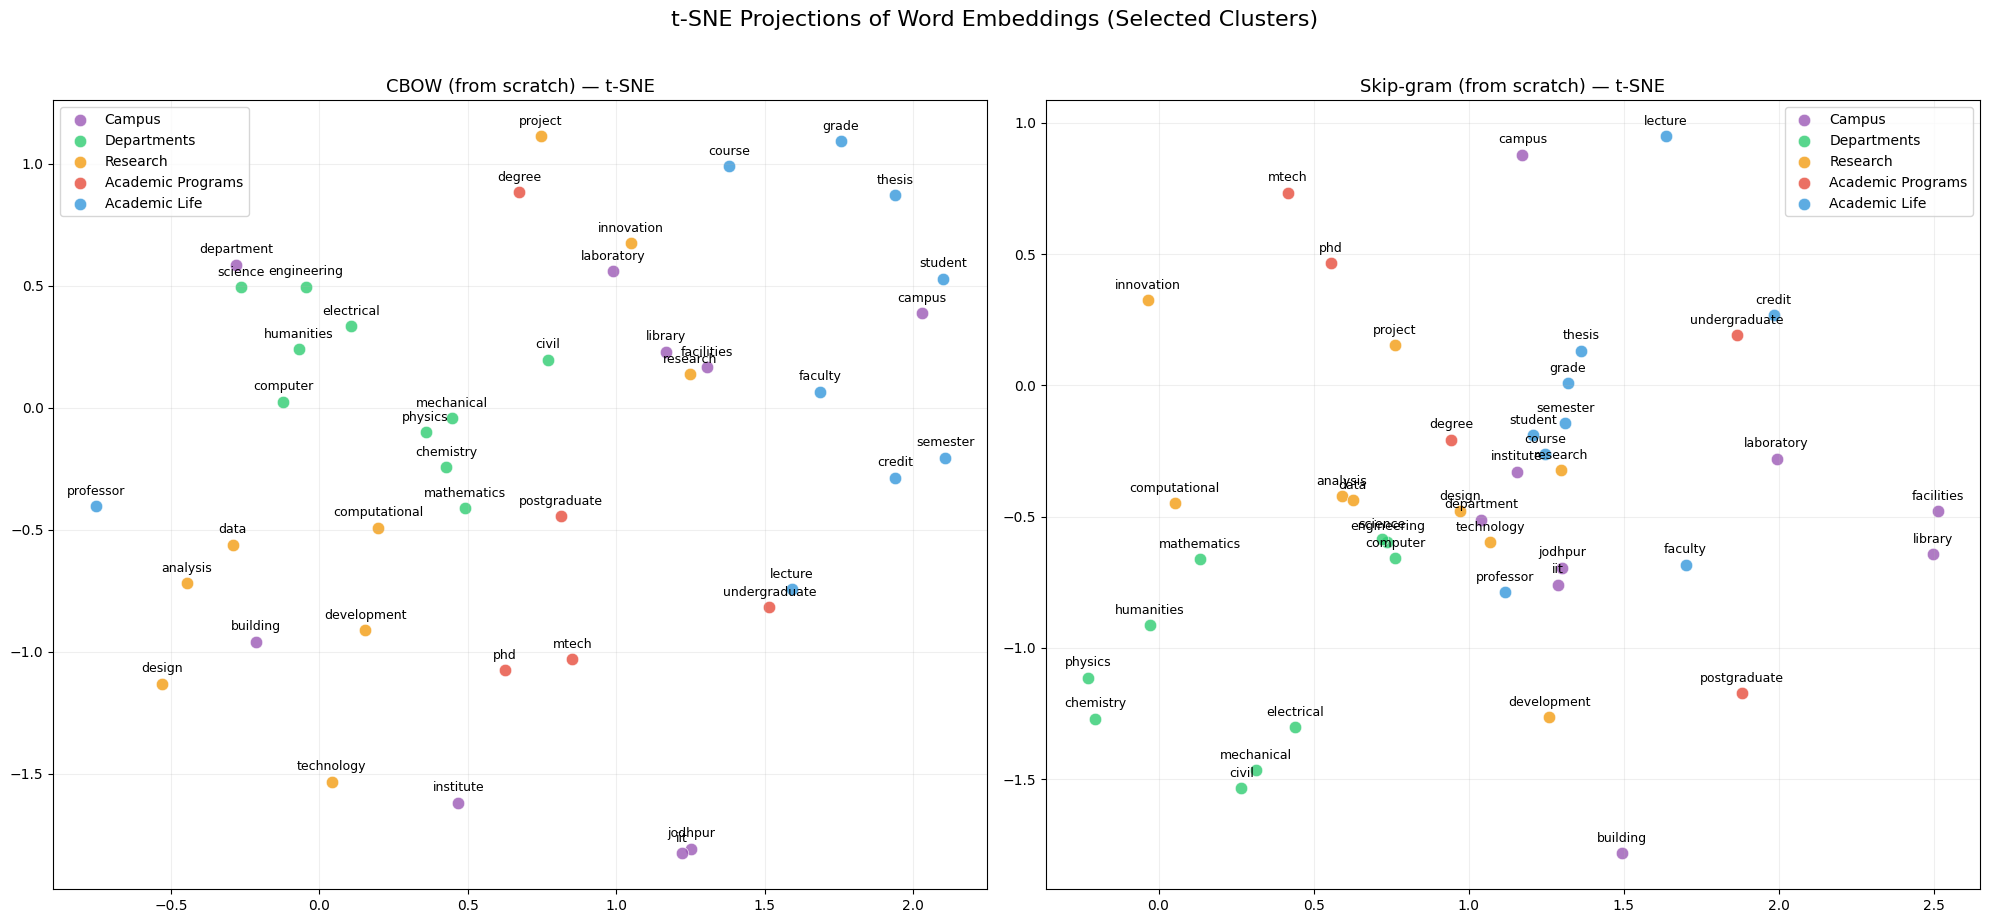
\includegraphics[width=\textwidth]{figures/t-SNE_Word_Embeddings.png}
\caption{t-SNE projections of selected word embeddings. Left: CBOW (from scratch). Right: Skip-gram (from scratch). Words are coloured by semantic category.}
\label{fig:tsne_scratch}
\end{figure}

\begin{figure}[H]
\centering
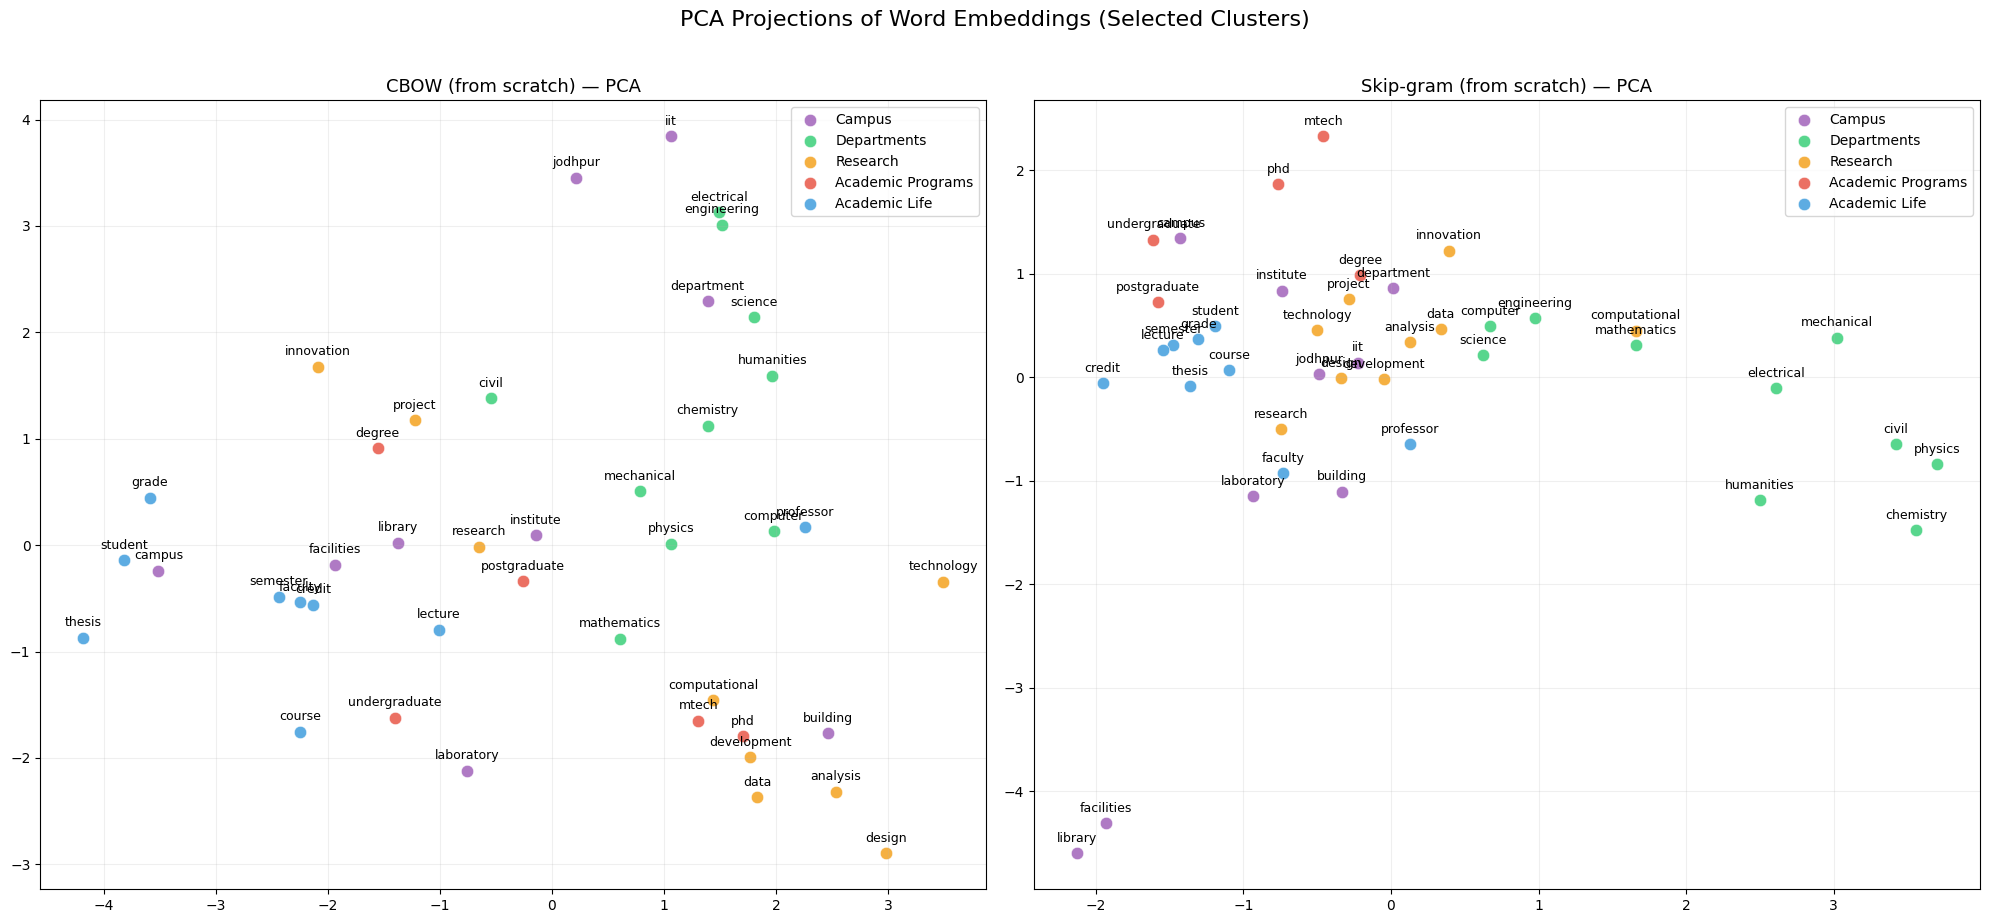
\includegraphics[width=\textwidth]{figures/PCA_word_embeddings.png}
\caption{PCA projections of selected word embeddings. Left: CBOW (from scratch). Right: Skip-gram (from scratch).}
\label{fig:pca_scratch}
\end{figure}

\begin{figure}[H]
\centering
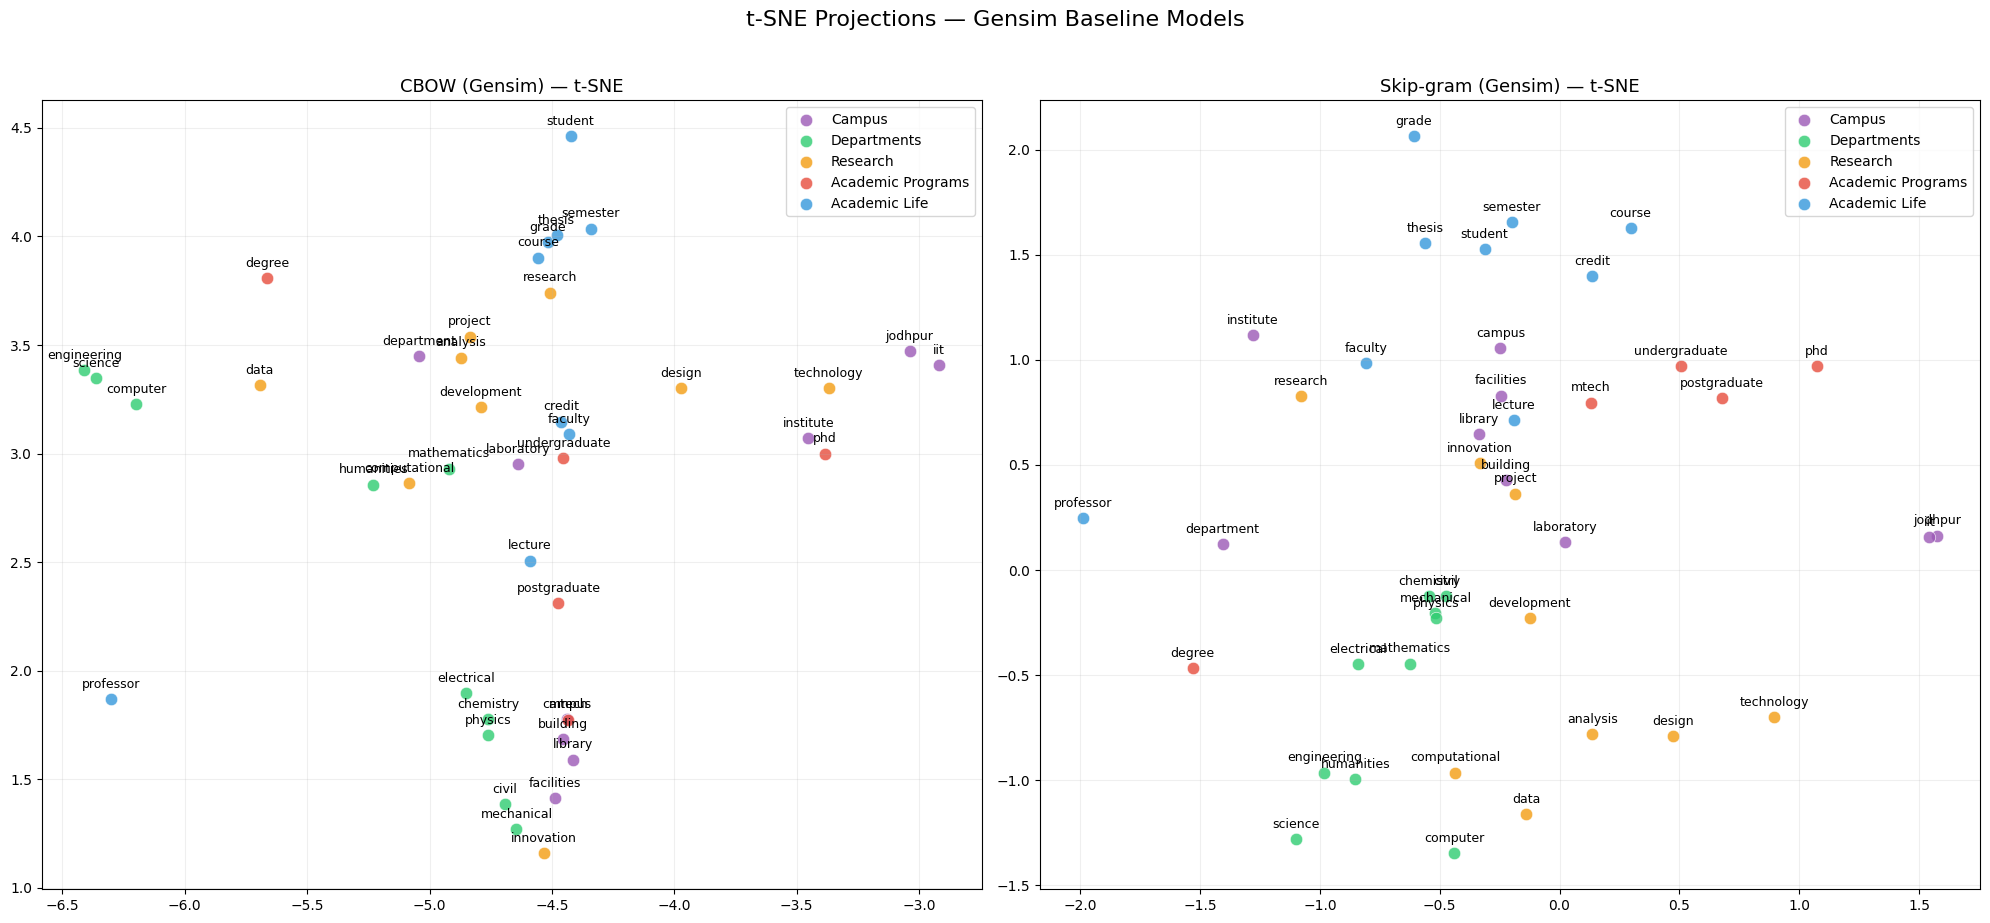
\includegraphics[width=\textwidth]{figures/Gensim_word_embeddings.png}
\caption{t-SNE projections for Gensim baseline models. Left: CBOW. Right: Skip-gram.}
\label{fig:tsne_gensim}
\end{figure}

\subsubsection{Interpretation}

In the t-SNE plots, several clusters are visually apparent. Department-related words (\emph{engineering}, \emph{computer}, \emph{electrical}, \emph{mechanical}) tend to group together, as do campus-related words (\emph{campus}, \emph{institute}, \emph{laboratory}). Academic life terms (\emph{semester}, \emph{grade}, \emph{credit}) also form a distinct neighbourhood, reflecting their co-occurrence in regulation documents.

Comparing CBOW and Skip-gram, the Skip-gram model produces more dispersed but semantically sharper clusters: words within the same category are close, while different categories maintain better separation. CBOW tends to produce tighter overall groupings but with more overlap between categories, because the context-averaging operation smooths out fine-grained distinctions.

The Gensim models exhibit cleaner separation overall, benefiting from subsampling of frequent words and optimised gradient updates that are absent in the from-scratch implementation.

% ======================================================================
%  PROBLEM 2
% ======================================================================
\newpage
\section{Problem 2: Character-Level Name Generation Using RNN Variants}

\subsection{Objective}

The goal of this problem is to design and compare sequence models for character-level name generation using three recurrent neural architectures: a Vanilla RNN, a Bidirectional LSTM (BLSTM), and an RNN with Bahdanau Attention. All recurrent cells are implemented from scratch using raw weight matrices; PyTorch is used only for activation functions (\texttt{torch.tanh}, \texttt{torch.sigmoid}), embeddings, the loss function, and the Adam optimiser. No \texttt{nn.RNN}, \texttt{nn.LSTM}, or \texttt{nn.GRU} modules are invoked.

% ─── Task 0 ───
\subsection{Task 0: Dataset}

A dataset of 1,000 unique Indian first names was assembled, covering a broad range of genders, regions (North, South, East, West India), and linguistic traditions (Hindi, Tamil, Telugu, Bengali, Marathi, Gujarati, Kannada, Malayalam, Punjabi, Odia). The names were generated in batches using a large language model and stored as \texttt{TrainingNames.txt}, one name per line.

\begin{table}[H]
\centering
\caption{Training dataset statistics.}
\label{tab:names_stats}
\begin{tabular}{lr}
\toprule
\textbf{Metric} & \textbf{Value} \\
\midrule
Total names          & 1,000 \\
Avg.\ name length    & 6.5 characters \\
Min / Max length     & 3 / 14 characters \\
Character vocabulary & 28 (25 letters\footnote{The letter `q' does not appear in the training names.} + \texttt{<PAD>} + \texttt{<SOS>} + \texttt{<EOS>}) \\
\bottomrule
\end{tabular}
\end{table}

\begin{figure}[H]
\centering
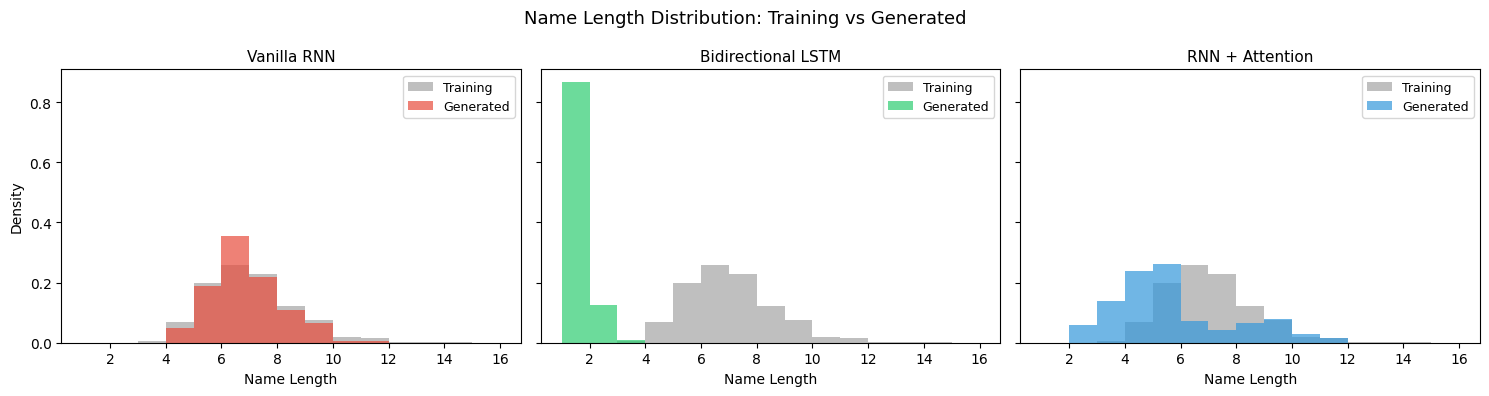
\includegraphics[width=0.95\textwidth]{figures/dl_name_length.png}
\caption{Left: Distribution of name lengths in the training set. The mode falls at 5--7 characters, consistent with typical Indian first names. Right: Character frequency distribution; the letter \emph{a} is by far the most common, appearing nearly four times as often as the next most frequent letter, reflecting its prevalence in Indian phonology.}
\label{fig:name_stats}
\end{figure}

Each name was encoded as a sequence of integer indices $[\texttt{SOS}, c_1, c_2, \ldots, c_n, \texttt{EOS}]$, and training pairs were formed as input $= [\texttt{SOS}, c_1, \ldots, c_n]$ and target $= [c_1, c_2, \ldots, c_n, \texttt{EOS}]$, yielding 1,000 training pairs.

% ─── Task 1 ───
\subsection{Task 1: Model Implementation}

All three models share the hyperparameters listed in Table~\ref{tab:rnn_hp}. Dropout was set to 0.3 to provide stronger regularisation against the overfitting risks inherent in a small 1,000-name dataset.

\begin{table}[H]
\centering
\caption{Shared hyperparameters for all three models.}
\label{tab:rnn_hp}
\begin{tabular}{lr}
\toprule
\textbf{Hyperparameter} & \textbf{Value} \\
\midrule
Embedding dimension & 64 \\
Hidden size         & 128 \\
Number of layers    & 2 \\
Dropout             & 0.3 \\
Learning rate       & 0.003 \\
Optimiser           & Adam \\
LR schedule         & StepLR (step=15, $\gamma$=0.5) \\
Batch size          & 64 \\
Epochs              & 100 \\
\bottomrule
\end{tabular}
\end{table}

\subsubsection{Model 1: Vanilla RNN}

The Vanilla RNN cell is implemented from scratch. At each timestep~$t$, it computes:
\begin{equation}
  h_t = \tanh\!\bigl(W_{ih}\, x_t + b_{ih} + W_{hh}\, h_{t-1} + b_{hh}\bigr)
\end{equation}

where $W_{ih} \in \mathbb{R}^{H \times d_{\mathrm{in}}}$, $W_{hh} \in \mathbb{R}^{H \times H}$, and $b_{ih}, b_{hh} \in \mathbb{R}^{H}$ are learnable parameters. Two such cells are stacked: Layer~1 maps from the embedding dimension ($64 \to 128$) and Layer~2 operates in hidden space ($128 \to 128$), with dropout applied between layers. A final linear projection maps from the hidden state to the vocabulary: $128 \to 28$.

\textbf{Total trainable parameters: 63,260.}

During generation, the model samples autoregressively starting from the \texttt{<SOS>} token. At each step, the hidden state is passed through the output projection, a softmax with temperature scaling produces a probability distribution over characters, and the next character is sampled. Generation terminates when \texttt{<EOS>} is produced or a maximum length is reached.

\subsubsection{Model 2: Bidirectional LSTM}

Each LSTM cell implements four gates from scratch using combined weight matrices for efficiency:
\begin{align}
  i_t &= \sigma(W_{ii}\, x + b_{ii} + W_{hi}\, h + b_{hi}) & &\text{(input gate)} \\
  f_t &= \sigma(W_{if}\, x + b_{if} + W_{hf}\, h + b_{hf}) & &\text{(forget gate)} \\
  g_t &= \tanh(W_{ig}\, x + b_{ig} + W_{hg}\, h + b_{hg}) & &\text{(cell gate)} \\
  o_t &= \sigma(W_{io}\, x + b_{io} + W_{ho}\, h + b_{ho}) & &\text{(output gate)} \\
  c_t &= f_t \odot c_{t-1} + i_t \odot g_t, \quad h_t = o_t \odot \tanh(c_t) \notag
\end{align}

The forget gate bias is initialised to 1.0 to encourage remembering at the start of training. At each layer, separate forward and backward LSTM cells process the sequence in opposite directions, and their outputs are concatenated to produce a $2H = 256$-dimensional representation. Two such bidirectional layers are stacked, with the output projected to the vocabulary: $256 \to 28$.

\textbf{Total trainable parameters: 602,908.}

\textit{Note on generation:} A bidirectional model inherently requires the full input sequence, since the backward pass reads from right to left. During autoregressive generation, the backward cells cannot be used as future characters are not yet available. Our generation strategy therefore uses only the forward LSTM cells, with the backward component zeroed out. This is a known and unavoidable compromise: the BLSTM learns richer bidirectional patterns during training, but generation is limited to the forward component only.

\subsubsection{Model 3: RNN with Bahdanau Attention}

The encoder consists of two stacked LSTM layers (from scratch, reusing the same \texttt{LSTMCell} as the BLSTM). At each decoding timestep~$t$, an additive (Bahdanau) attention mechanism computes alignment scores over all encoder hidden states:
\begin{align}
  e_{t,s} &= \mathbf{v}^\top \tanh(W_q\, h_t + W_k\, h_s), \quad \forall \text{ source positions } s \\
  \alpha_t &= \mathrm{softmax}(e_t) \\
  \mathrm{context} &= \textstyle\sum_s \alpha_{t,s}\, h_s
\end{align}

where $W_q, W_k \in \mathbb{R}^{H \times H}$ and $\mathbf{v} \in \mathbb{R}^{H}$ are learnable attention parameters. The concatenation $[h_t;\, \mathrm{context}]$ (dimension $2H = 256$) is projected to the vocabulary.

\textbf{Total trainable parameters: 273,308.}

During generation, the full sequence of characters generated so far is re-encoded at each step, and the attention mechanism attends over the encoder outputs to produce the next character. This re-encoding strategy, while faithful to the attention architecture, is computationally expensive and introduces a train--test mismatch that contributes to the generation difficulties discussed below.

\begin{table}[H]
\centering
\caption{Parameter count comparison across the three models.}
\label{tab:param_counts}
\begin{tabular}{lr}
\toprule
\textbf{Model} & \textbf{Trainable Parameters} \\
\midrule
Vanilla RNN        &  63,260 \\
Bidirectional LSTM & 602,908 \\
RNN + Attention    & 273,308 \\
\bottomrule
\end{tabular}
\end{table}

% ─── Training ───
\subsection{Training Results}

All three models were trained for 100 epochs on the 1,000 training pairs. Figure~\ref{fig:rnn_loss} shows the training loss curves, and Table~\ref{tab:training_epochs} provides epoch-level detail.

\begin{figure}[H]
\centering
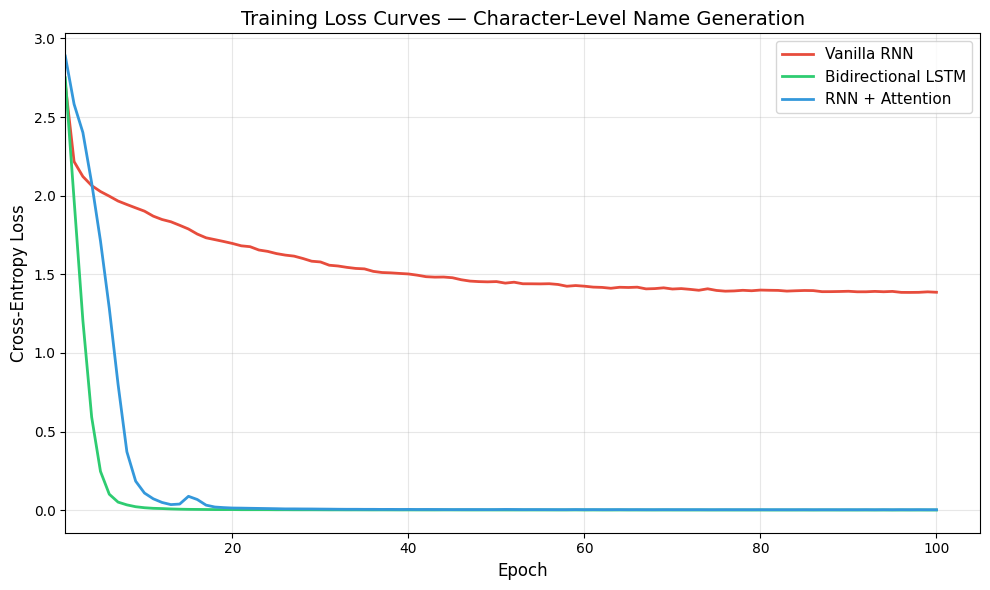
\includegraphics[width=0.85\textwidth]{figures/training_loss_dl.png}
\caption{Training loss curves over 100 epochs. The Vanilla RNN converges gradually to a loss of 1.39, suggesting it has learned generalisable patterns. The BLSTM and Attention models collapse to near-zero loss rapidly, indicating memorisation of the training data.}
\label{fig:rnn_loss}
\end{figure}

\begin{table}[H]
\centering
\caption{Training loss at selected epochs with representative generated samples.}
\label{tab:training_epochs}
\small
\begin{tabular}{clp{8.5cm}}
\toprule
\textbf{Epoch} & \textbf{Loss} & \textbf{Sample Names} \\
\midrule
\multicolumn{3}{l}{\textit{Vanilla RNN}} \\
1   & 2.7103 & Rokannt, Nanshi, Gewminie, Tara, Mamabi \\
10  & 1.9018 & Ashudhka, Urdeep, Seminder, Sama, Charitra \\
30  & 1.5578 & Bhanvi, Parvi, Parmun, Chantuli, Kappala \\
60  & 1.4245 & Praveen, Ramani, Devpreet, Sumitha, Swothi \\
100 & 1.3859 & Sindil, Manesh, Charuta, Sojan, Piha \\
\midrule
\multicolumn{3}{l}{\textit{Bidirectional LSTM}} \\
1   & 2.7498 & Gemlh, Ejthi, Guece, Ramv, Tifea \\
10  & 0.0155 & A, (empty), P, (empty), H \\
50  & 0.0013 & Ut, W, (empty), Wu, (empty) \\
100 & 0.0010 & (empty), B, F, D, (empty) \\
\midrule
\multicolumn{3}{l}{\textit{RNN + Attention}} \\
1   & 2.8884 & Suiaadaau, N, Ikialhaa, Hkds, Hialan \\
10  & 0.1088 & Fevvy, Jjjjj, Mm, (empty), Mmmm \\
50  & 0.0038 & Ppppp, Ffwwwww, Aar, Ii, (empty) \\
100 & 0.0027 & Aaa, Ffwwwfwww, Mmmmm, (empty), (empty) \\
\bottomrule
\end{tabular}
\end{table}

\paragraph{Vanilla RNN.} This model displayed healthy, gradual convergence from 2.71 to 1.39 over 100 epochs. The generated samples improved systematically: early outputs (\emph{Rokannt}, \emph{Gewminie}) were gibberish, mid-training names (\emph{Bhanvi}, \emph{Charitra}) showed clear Indian phonotactics, and final outputs (\emph{Praveen}, \emph{Ramani}, \emph{Devpreet}) were largely indistinguishable from real names. The dropout rate of 0.3 provided sufficient regularisation to prevent the loss from collapsing to zero, forcing the model to learn generalisable character-level patterns rather than memorising individual names.

\paragraph{Bidirectional LSTM.} Despite starting at a comparable loss (2.75), the BLSTM collapsed to 0.015 by epoch~10 and reached 0.001 by epoch~50. This near-zero training loss indicates total memorisation. During generation, the forward-only cells (with backward cells zeroed) lack the bidirectional context they were trained with, producing mostly empty strings or isolated characters. The model's 602,908 parameters---nearly ten times those of the Vanilla RNN---provide far more capacity than needed for 1,000 short names, making overfitting inevitable despite the 0.3 dropout rate.

\paragraph{RNN + Attention.} This model followed a similar trajectory: loss dropped from 2.89 to 0.003 within 50 epochs. The attention mechanism exacerbated overfitting because it allows the model to perfectly reconstruct any training sequence by learning to attend to the correct positions. During generation, the re-encoding strategy creates a distribution shift: the model sees its own noisy outputs rather than clean training data, causing the attention to lock onto single characters and repeat them (``Ppppp'', ``Mmmm'', ``Ffwwwfwww'').

% ─── Task 2 ───
\subsection{Task 2: Quantitative Evaluation}

Two hundred names were generated per model at temperature 0.8. Names that were empty strings were excluded from the count. Table~\ref{tab:quant_eval} reports the metrics.

\textbf{Novelty Rate} is defined as the percentage of generated names that do not appear in the training set. \textbf{Diversity} is the number of unique generated names divided by the total generated names.

\begin{table}[H]
\centering
\caption{Quantitative evaluation of generated names (200 attempts per model, temperature = 0.8).}
\label{tab:quant_eval}
\begin{tabular}{lrrrcc}
\toprule
\textbf{Model} & \textbf{Params} & \textbf{Total} & \textbf{Unique} & \textbf{Novelty (\%)} & \textbf{Diversity (\%)} \\
\midrule
Vanilla RNN        &  63,260 & 200 & 189 & 69.0 & 94.5 \\
Bidirectional LSTM & 602,908 & 112 &  26 & 23.2 & 23.2 \\
RNN + Attention    & 273,308 & 139 &  61 & 43.9 & 43.9 \\
\bottomrule
\end{tabular}
\end{table}

\begin{figure}[H]
\centering
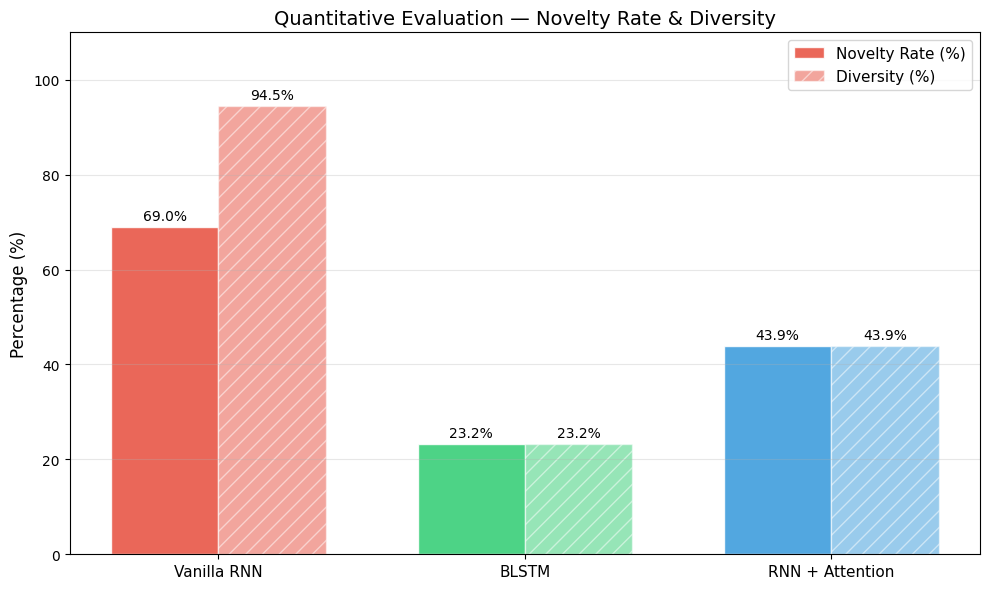
\includegraphics[width=0.85\textwidth]{figures/novelty_rate_diversity.png}
\caption{Novelty rate and diversity comparison. The Vanilla RNN dominates both metrics, producing nearly all valid names with 94.5\% diversity and 69\% novelty.}
\label{fig:quant_bar}
\end{figure}

\paragraph{Analysis.} The Vanilla RNN produced all 200 valid names with 189 unique outputs (94.5\% diversity). Of these, 138 were novel---names not present in the training set at all---yielding a novelty rate of 69\%. This is an excellent result: the model has learned to generalise from the training data to produce new, phonetically plausible Indian names while still being capable of reproducing real ones.

The BLSTM produced only 112 non-empty outputs from 200 attempts (the rest were empty strings), with just 26 unique names. All 26 unique outputs were novel, but only because they were meaningless fragments (single characters or two-character strings) that trivially differ from any training name.

The Attention model produced 139 non-empty outputs with 61 unique names. Again, all unique outputs were technically novel, but most consisted of repeated character patterns rather than plausible names. The equal novelty and diversity percentages for both BLSTM and Attention models (23.2\% and 43.9\% respectively) reflect the fact that their unique outputs are entirely novel but degenerate.

% ─── Task 3 ───
\subsection{Task 3: Qualitative Analysis}

\subsubsection{Representative Samples}

\paragraph{Vanilla RNN.} The model generates a rich mix of novel but phonetically plausible names alongside recognisable training names:

\begin{itemize}[nosep]
  \item \textbf{Novel names (23 of 30 samples):} Gourdhan, Sudama, Sreejanta, Pravith, Harshar, Ajvinder, Sheema, Balabasarta, Anshara, Sitali, Amarita, Bitali, Bhavi, Samaraj, Kishuja, Shati, Misha, Amurta, Pramandeet
  \item \textbf{Names also in training set (7 of 30):} Bhavika, Sandhya, Shantala, Amit, Deepa, Praveena, Abhilash
\end{itemize}

The novel names demonstrate that the model has internalised the phonotactic structure of Indian names: common prefixes (\emph{An-}, \emph{Pra-}, \emph{Sree-}), productive suffixes (\emph{-ita}, \emph{-deet}, \emph{-inder}, \emph{-ama}), vowel-consonant alternation patterns, and the typical length distribution of 4--9 characters.

\paragraph{Bidirectional LSTM.} The 30 generated samples consisted almost entirely of single characters or two-character fragments: G, Ko, P, E, Gs, F, D, K, H, S, Sy, Gk, Wu, Ut, W, etc. The forward-only generation cannot reconstruct the rich representations that the bidirectional training produced, and the model terminates almost immediately after the start token.

\paragraph{RNN + Attention.} Outputs exhibit pathological character repetition: Aaa, Ppppp, Mmmm, Gggg, Rrrrr, Chhhh, Ffwwwfwww, Bbbbbbbb. The attention mechanism, trained to perfectly reconstruct sequences, gets locked into attending to a single character position when faced with its own noisy outputs during autoregressive generation.

\subsubsection{Common Failure Modes}

\begin{table}[H]
\centering
\caption{Summary of observed failure modes across models.}
\label{tab:failures}
\small
\begin{tabular}{p{3.5cm}p{3cm}p{6cm}}
\toprule
\textbf{Failure Mode} & \textbf{Affected Models} & \textbf{Description} \\
\midrule
Empty / single-char outputs & BLSTM & Forward-only generation lacks backward context; model produces \texttt{<EOS>} almost immediately. \\
Character repetition loops & Attention & Attention locks onto one position, repeating a single character (e.g., ``Ppppp'', ``Mmmm''). \\
Unusual consonant clusters & Vanilla RNN & Occasional outputs like ``Thrit'' or ``Kappala'' with atypical sequences, though still phonetically attempted. \\
Near-zero training loss & BLSTM, Attention & Both models memorise the training set completely, losing the ability to generalise during generation. \\
\bottomrule
\end{tabular}
\end{table}

\begin{figure}[H]
\centering
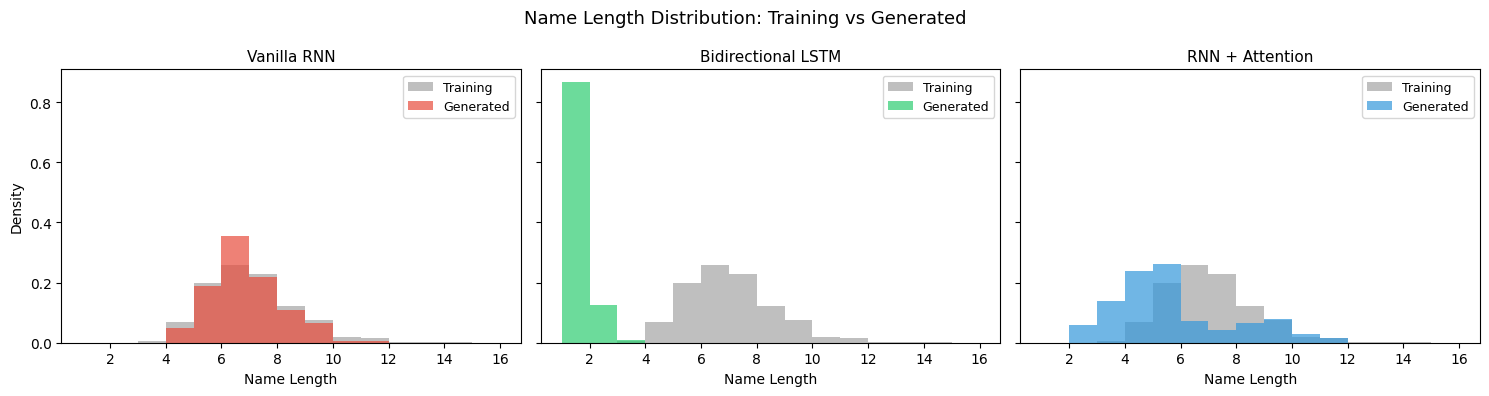
\includegraphics[width=\textwidth]{figures/dl_name_length.png}
\caption{Name length distributions of generated names (blue) vs.\ training data (grey). The Vanilla RNN closely approximates the training distribution, while the BLSTM produces extremely short outputs and the Attention model generates names with an anomalous length profile dominated by repeated characters.}
\label{fig:length_dist}
\end{figure}

\subsubsection{Temperature Effects}

Temperature was varied on the RNN + Attention model to investigate whether the repetition problem could be mitigated. As Table~\ref{tab:temp_effect} shows, all temperature settings produce degenerate outputs, confirming that the problem is structural (overfitting and train--test mismatch) rather than a sampling artefact.

\begin{table}[H]
\centering
\caption{Temperature effects on RNN + Attention generation. The repetition pathology persists across all settings.}
\label{tab:temp_effect}
\small
\begin{tabular}{cp{9cm}}
\toprule
\textbf{Temp.} & \textbf{Samples} \\
\midrule
0.5 & (empty), Cccccccccccchchhhh, Ppppp, (empty), Mmmm \\
0.8 & Hhhh, Kkkkk, (empty), Mmmm, Ffffwwfwff \\
1.0 & Rrrrrrr, Ppppp, Pppp, Ppppp, Mmmmm \\
1.2 & Rrrrrrr, (empty), Uuu, Ffeee, Fooo, Aaa \\
\bottomrule
\end{tabular}
\end{table}

At low temperature (0.5), the model produces more empty outputs (the argmax path leads directly to \texttt{<EOS>}). At high temperature (1.2), there is slightly more character variety, but the fundamental repetition pattern remains. This confirms that the attention mechanism's failure is not a matter of sampling strategy but of the model's inability to produce coherent sequences autoregressively after having been trained on perfect teacher-forced inputs.

% ─── Summary ───
\subsection{Summary and Discussion}

\begin{table}[H]
\centering
\caption{Overall comparison of the three architectures for character-level name generation.}
\label{tab:rnn_summary}
\small
\begin{tabular}{lccc}
\toprule
\textbf{Aspect} & \textbf{Vanilla RNN} & \textbf{BLSTM} & \textbf{RNN + Attention} \\
\midrule
Parameters          & 63K      & 603K     & 273K \\
Best training loss  & 1.385    & 0.0009   & 0.0026 \\
Valid outputs (of 200) & 200   & 112      & 139 \\
Diversity           & 94.5\%   & 23.2\%   & 43.9\% \\
Novelty             & 69.0\%   & 23.2\%   & 43.9\% \\
Sample quality      & Excellent & Poor (fragments) & Poor (repetitions) \\
Primary issue       & ---      & Forward-only gap & Attention collapse \\
\bottomrule
\end{tabular}
\end{table}

The central finding of this study is that the simplest model---the Vanilla RNN with just 63,260 parameters---dramatically outperformed both the Bidirectional LSTM and the RNN with Attention on every practical metric: valid output rate, diversity, novelty, and qualitative realism.

The BLSTM and Attention models illustrate two distinct but related failure patterns. The BLSTM fails because its training and generation regimes are fundamentally mismatched: during training it sees the full sequence from both directions, but during generation it can only operate in the forward direction, losing the backward context that accounts for half of its learned representation. The Attention model fails through a different mechanism: it overfits by learning to perfectly reconstruct training sequences via precise attention patterns, but during autoregressive generation the accumulation of its own errors (exposure bias) causes the attention to degenerate into repetitive loops.

These results highlight an important principle in sequence modelling: \emph{more complex architectures are not universally better}. For small datasets (1,000 names) and relatively simple sequential tasks (character-level generation of short strings), a lightweight Vanilla RNN with appropriate regularisation (dropout = 0.3) provides the optimal balance between learning capacity and generalisation ability. The more powerful models would likely require significantly larger training datasets, curriculum learning, scheduled sampling, or other techniques to overcome their overfitting tendencies on data of this scale.

% ======================================================================
%  REFERENCES
% ======================================================================
\newpage
\section*{References}
\addcontentsline{toc}{section}{References}

\begin{enumerate}[label={[\arabic*]}]
  \item T.\ Mikolov, K.\ Chen, G.\ Corrado, and J.\ Dean, ``Efficient Estimation of Word Representations in Vector Space,'' \textit{ICLR Workshop}, 2013.
  \item T.\ Mikolov, I.\ Sutskever, K.\ Chen, G.\ Corrado, and J.\ Dean, ``Distributed Representations of Words and Phrases and their Compositionality,'' \textit{NeurIPS}, 2013.
  \item Y.\ Goldberg and O.\ Levy, ``word2vec Explained,'' \textit{arXiv:1402.3722}, 2014.
  \item J.\ L.\ Elman, ``Finding Structure in Time,'' \textit{Cognitive Science}, vol.\ 14, no.\ 2, pp.\ 179--211, 1990.
  \item S.\ Hochreiter and J.\ Schmidhuber, ``Long Short-Term Memory,'' \textit{Neural Computation}, vol.\ 9, no.\ 8, pp.\ 1735--1780, 1997.
  \item M.\ Schuster and K.\ K.\ Paliwal, ``Bidirectional Recurrent Neural Networks,'' \textit{IEEE Trans.\ Signal Processing}, vol.\ 45, no.\ 11, 1997.
  \item D.\ Bahdanau, K.\ Cho, and Y.\ Bengio, ``Neural Machine Translation by Jointly Learning to Align and Translate,'' \textit{ICLR}, 2015.
\end{enumerate}

\end{document}
